%%
%% Automatically generated file from DocOnce source
%% (https://github.com/hplgit/doconce/)
%%
%%
% #ifdef PTEX2TEX_EXPLANATION
%%
%% The file follows the ptex2tex extended LaTeX format, see
%% ptex2tex: http://code.google.com/p/ptex2tex/
%%
%% Run
%%      ptex2tex myfile
%% or
%%      doconce ptex2tex myfile
%%
%% to turn myfile.p.tex into an ordinary LaTeX file myfile.tex.
%% (The ptex2tex program: http://code.google.com/p/ptex2tex)
%% Many preprocess options can be added to ptex2tex or doconce ptex2tex
%%
%%      ptex2tex -DMINTED myfile
%%      doconce ptex2tex myfile envir=minted
%%
%% ptex2tex will typeset code environments according to a global or local
%% .ptex2tex.cfg configure file. doconce ptex2tex will typeset code
%% according to options on the command line (just type doconce ptex2tex to
%% see examples). If doconce ptex2tex has envir=minted, it enables the
%% minted style without needing -DMINTED.
% #endif

% #define PREAMBLE

% #ifdef PREAMBLE
%-------------------- begin preamble ----------------------

\documentclass[%
twoside,                 % oneside: electronic viewing, twoside: printing
final,                   % or draft (marks overfull hboxes, figures with paths)
10pt]{article}

\listfiles               % print all files needed to compile this document

\usepackage{relsize,makeidx,color,setspace,amsmath,amsfonts}
\usepackage[table]{xcolor}
\usepackage{bm,microtype}

\usepackage{graphicx}

\usepackage[T1]{fontenc}
%\usepackage[latin1]{inputenc}
\usepackage{ucs}
\usepackage[utf8x]{inputenc}

\usepackage{lmodern}         % Latin Modern fonts derived from Computer Modern

% Hyperlinks in PDF:
\definecolor{linkcolor}{rgb}{0,0,0.4}
\usepackage{hyperref}
\hypersetup{
    breaklinks=true,
    colorlinks=true,
    linkcolor=linkcolor,
    urlcolor=linkcolor,
    citecolor=black,
    filecolor=black,
    %filecolor=blue,
    pdfmenubar=true,
    pdftoolbar=true,
    bookmarksdepth=3   % Uncomment (and tweak) for PDF bookmarks with more levels than the TOC
    }
%\hyperbaseurl{}   % hyperlinks are relative to this root

\setcounter{tocdepth}{2}  % number chapter, section, subsection

% Tricks for having figures close to where they are defined:
% 1. define less restrictive rules for where to put figures
\setcounter{topnumber}{2}
\setcounter{bottomnumber}{2}
\setcounter{totalnumber}{4}
\renewcommand{\topfraction}{0.85}
\renewcommand{\bottomfraction}{0.85}
\renewcommand{\textfraction}{0.15}
\renewcommand{\floatpagefraction}{0.7}
% 2. ensure all figures are flushed before next section
\usepackage[section]{placeins}
% 3. enable begin{figure}[H] (often leads to ugly pagebreaks)
%\usepackage{float}\restylefloat{figure}

\usepackage[framemethod=TikZ]{mdframed}

% --- begin definitions of admonition environments ---

% --- end of definitions of admonition environments ---

% prevent orhpans and widows
\clubpenalty = 10000
\widowpenalty = 10000

% --- end of standard preamble for documents ---


% insert custom LaTeX commands...

\raggedbottom
\makeindex

%-------------------- end preamble ----------------------

\begin{document}

% endif for #ifdef PREAMBLE
% #endif


% ------------------- main content ----------------------



% ----------------- title -------------------------

\thispagestyle{empty}

\begin{center}
{\LARGE\bf
\begin{spacing}{1.25}
Education for the future
\end{spacing}
}
\end{center}

% ----------------- author(s) -------------------------

\begin{center}
{\bf Morten Hjorth-Jensen${}^{1, 2}$} \\ [0mm]
\end{center}

    
\begin{center}
{\bf Anders Malthe-Sørenssen${}^{1}$} \\ [0mm]
\end{center}

    \begin{center}
% List of all institutions:
\centerline{{\small ${}^1$Department of Physics, University of Oslo}}
\centerline{{\small ${}^2$Department of Physics and Astronomy, Michigan State University, USA}}
\end{center}
    
% ----------------- end author(s) -------------------------

\begin{center} % date
September 2 2015,
\end{center}

\vspace{1cm}


% !split
\subsection{Present and future education}

% --- begin paragraph admon ---
\paragraph{}

\begin{itemize}
\item \textbf{Research-based education}, from undergraduate studies to a PhD: \href{{http://www.mn.uio.no/fysikk/english/research/groups/computational/index.html}}{The Computational Physics group at the University of Oslo} as example

\item Future challenges and directions
\end{itemize}

\noindent
% --- end paragraph admon ---



% --- begin paragraph admon ---
\paragraph{Takeaway message.}
Excellent research mutually depends on excellent education.
% A successful research program cannot be disconnected from education and vice versa
% --- end paragraph admon ---



% !split
\subsection{The role of computations, from education to society}

% --- begin paragraph admon ---
\paragraph{}
\textbf{Computations are central to our 
basic understanding of nature and to technological advances}.
UiO's strength in computational science (education and research)
has the potential to make UiO a top European university.
% --- end paragraph admon ---




% --- begin paragraph admon ---
\paragraph{Examples.}
\begin{itemize}
\item \textbf{Nanotech and Materials}: quantum physical systems in nanotechnology; characteristics of new materials; semi-conductor devices and quantum computers

\item \textbf{The smallest particles in nature}: subatomic physics at its smallest length scale

\item \textbf{And the largest}: simulating galaxies and the evolution of the universe

\item \textbf{Life science}: cancer treatment and how the brain works

\item \textbf{Geosciences}: predicting climate changes and this week's weather, simulating natural disasters

\item \textbf{Finance}: assessing risk in the insurance and financial industry

\item and many many more
\end{itemize}

\noindent
% --- end paragraph admon ---



% !split
\subsection{Modeling and computations as a way to enhance algorithminc thinking}


% --- begin paragraph admon ---
\paragraph{}
\textbf{Algorithm} :
A set of instructions to solve a problem.
% --- end paragraph admon ---




% --- begin paragraph admon ---
\paragraph{Algorithmic thinking applies to all disciplines. It.}
\begin{itemize}
\item Enhances instruction-based teaching

\item Introduces research-based teaching  from day one

\item Triggers further insights in scientific problems

\item Emphasizes validation and verification of scientific results, and integrates science ethics in a natural way

\item Ensures good working practices from day one!
\end{itemize}

\noindent
% --- end paragraph admon ---





% !split
\subsection{What does computing mean?}


% --- begin paragraph admon ---
\paragraph{}

\textbf{Computing means solving scientific problems using computers. It covers numerical as well as symbolic computing. Computing is also about developing an understanding of the scientific process by enhancing the algorithmic thinking when solving problems.}
% --- end paragraph admon ---




% --- begin paragraph admon ---
\paragraph{Computing competence is about:}

\begin{itemize}
\item derivation, verification, and implementation of algorithms

\item understanding what can go wrong with algorithms

\item overview of important, known algorithms

\item understanding how algorithms are used to solve complicated problems

\item reproducible science and ethics

\item algorithmic thinking for gaining deeper insights about scientific problems
\end{itemize}

\noindent
All these elements (and many more) aid students in maturing and gaining a better understanding of the scientific process \emph{per se}.
% --- end paragraph admon ---







% !split
\subsection{Computing and research-based education}


% --- begin paragraph admon ---
\paragraph{}
A computational approach allows us to introduce research concepts and engage students in research from \emph{day one}.
% --- end paragraph admon ---





% --- begin paragraph admon ---
\paragraph{What should the education contain?}

\begin{itemize}
\item Theory + experiment + simulation is the norm in research and industry

\item Modeling of real, complex systems with no simple answers

\item Insight and understanding of fundamental principles and laws

\item Visualization, presentation, discussion, interpretation, and critical analysis of results

\item Development of a sound ethical attitude to own and other's work

\item Enhanced reasoning about the scientific method

\item Individually tailored education in order to let students  realize their full potentials and discover their creative powers
\end{itemize}

\noindent
This is what we do in the \href{{http://www.mn.uio.no/fysikk/english/research/groups/computational/index.html}}{Computational Physics group at UiO}!
% --- end paragraph admon ---




% !split
\subsection{\href{{http://www.mn.uio.no/fysikk/english/research/groups/computational/index.html}}{Computational Physics group at UiO}; our visions}

% !bslidecell 00 0.4

% --- begin paragraph admon ---
\paragraph{}
Physics students can \textbf{pose and solve problems} that combine \textbf{physical insights} with \textbf{mathematical tools} and now also \textbf{computational skills}. This provides a unique combination of applied and theoretical knowledge and skills. These features are invaluable for the development of multi-disciplinary educational and research programs.
% --- end paragraph admon ---


% !eslidecell

% !bslidecell 01 0.6


% inline figure
\centerline{
\includegraphics[width=1.0\linewidth]{fig-future/computer_nerd2.jpg}}


% !eslidecell


% !split
\subsection{A social and scientific learning environment}


% --- begin paragraph admon ---
\paragraph{}
\textbf{Goal: Students should realize their full potentials and discover their creative powers}

\begin{itemize}
 \item Students come with different dreams, ambitions, aspirations and topics they wish to study, our approach is to tailor the education to all these aspects

 \item Our motto: foster students who are better than their supervisors

 \item Emphasis is on learning and getting new insights

 \item Students and teachers help each other

 \item Students with different backgrounds and needs can thrive socially and scientifically

 \item Not a competitive environment, but a drive and enthusiam for sharing and developing knowledge. This is an important element for the  success of for example multi-disciplinary projects 
\end{itemize}

\noindent
% --- end paragraph admon ---





% !split
\subsection{We develop a social and scientific learning environment}


% --- begin paragraph admon ---
\paragraph{}
\begin{itemize}
\item We target bachelor, MSc and PhD students

\item Project-oriented work where students develop and mature their own ideas, with an individually tailored approach to each student

\item Office space with desktops to every student and large common room for recreational activities (meals, gaming, movies)

\item Many students collaborate on similar  thesis topics and \href{{http://www.dn.no/talent/2014/06/12/Utdannelse/sommervikar-ble-toppforsker}}{publish in top scientific journals}
\end{itemize}

\noindent
% --- end paragraph admon ---





% !split
\subsection{Features of the Computational Physics group}

% --- begin paragraph admon ---
\paragraph{}
\begin{itemize}
\item Our students have made significant contributions to  the \href{{http://www.mn.uio.no/english/about/collaboration/cse/}}{Computing in Science Education}  (UiO education prize in 2011) by developing exercises and participating in educational projects at the MN faculty

\item Our students have also developed educational \href{{http://www.mn.uio.no/fysikk/om/aktuelt/aktuelle-saker/2015/realfagsapper.html}}{tools and applications for understanding complicated physical problems}

\item A group of PhD students is now developing \href{{https://github.com/CINPLA/ibvcse}}{new textbooks for Computational Life Science}

\item 2005-2015: $> 60$ students have finalized their master's theses and 60\% have continued with PhD studies

\item Many students don't want to leave the group after finishing their studies
\end{itemize}

\noindent
% --- end paragraph admon ---






% !split
\subsection{Investing in equipment for research and education}
% !bslidecell 00 0.2

% --- begin paragraph admon ---
\paragraph{}
Large screens for visualizing and presenting scientific results. And gaming and other social activities. 
\begin{itemize}
\item Here we see two students displaying results from large-scale simulations of molecules in materials

\item With 3D visualization tools one can see structures which where not possible until recently
\end{itemize}

\noindent
% --- end paragraph admon ---


% !eslidecell

% !bslidecell 01 0.8


% inline figure
\centerline{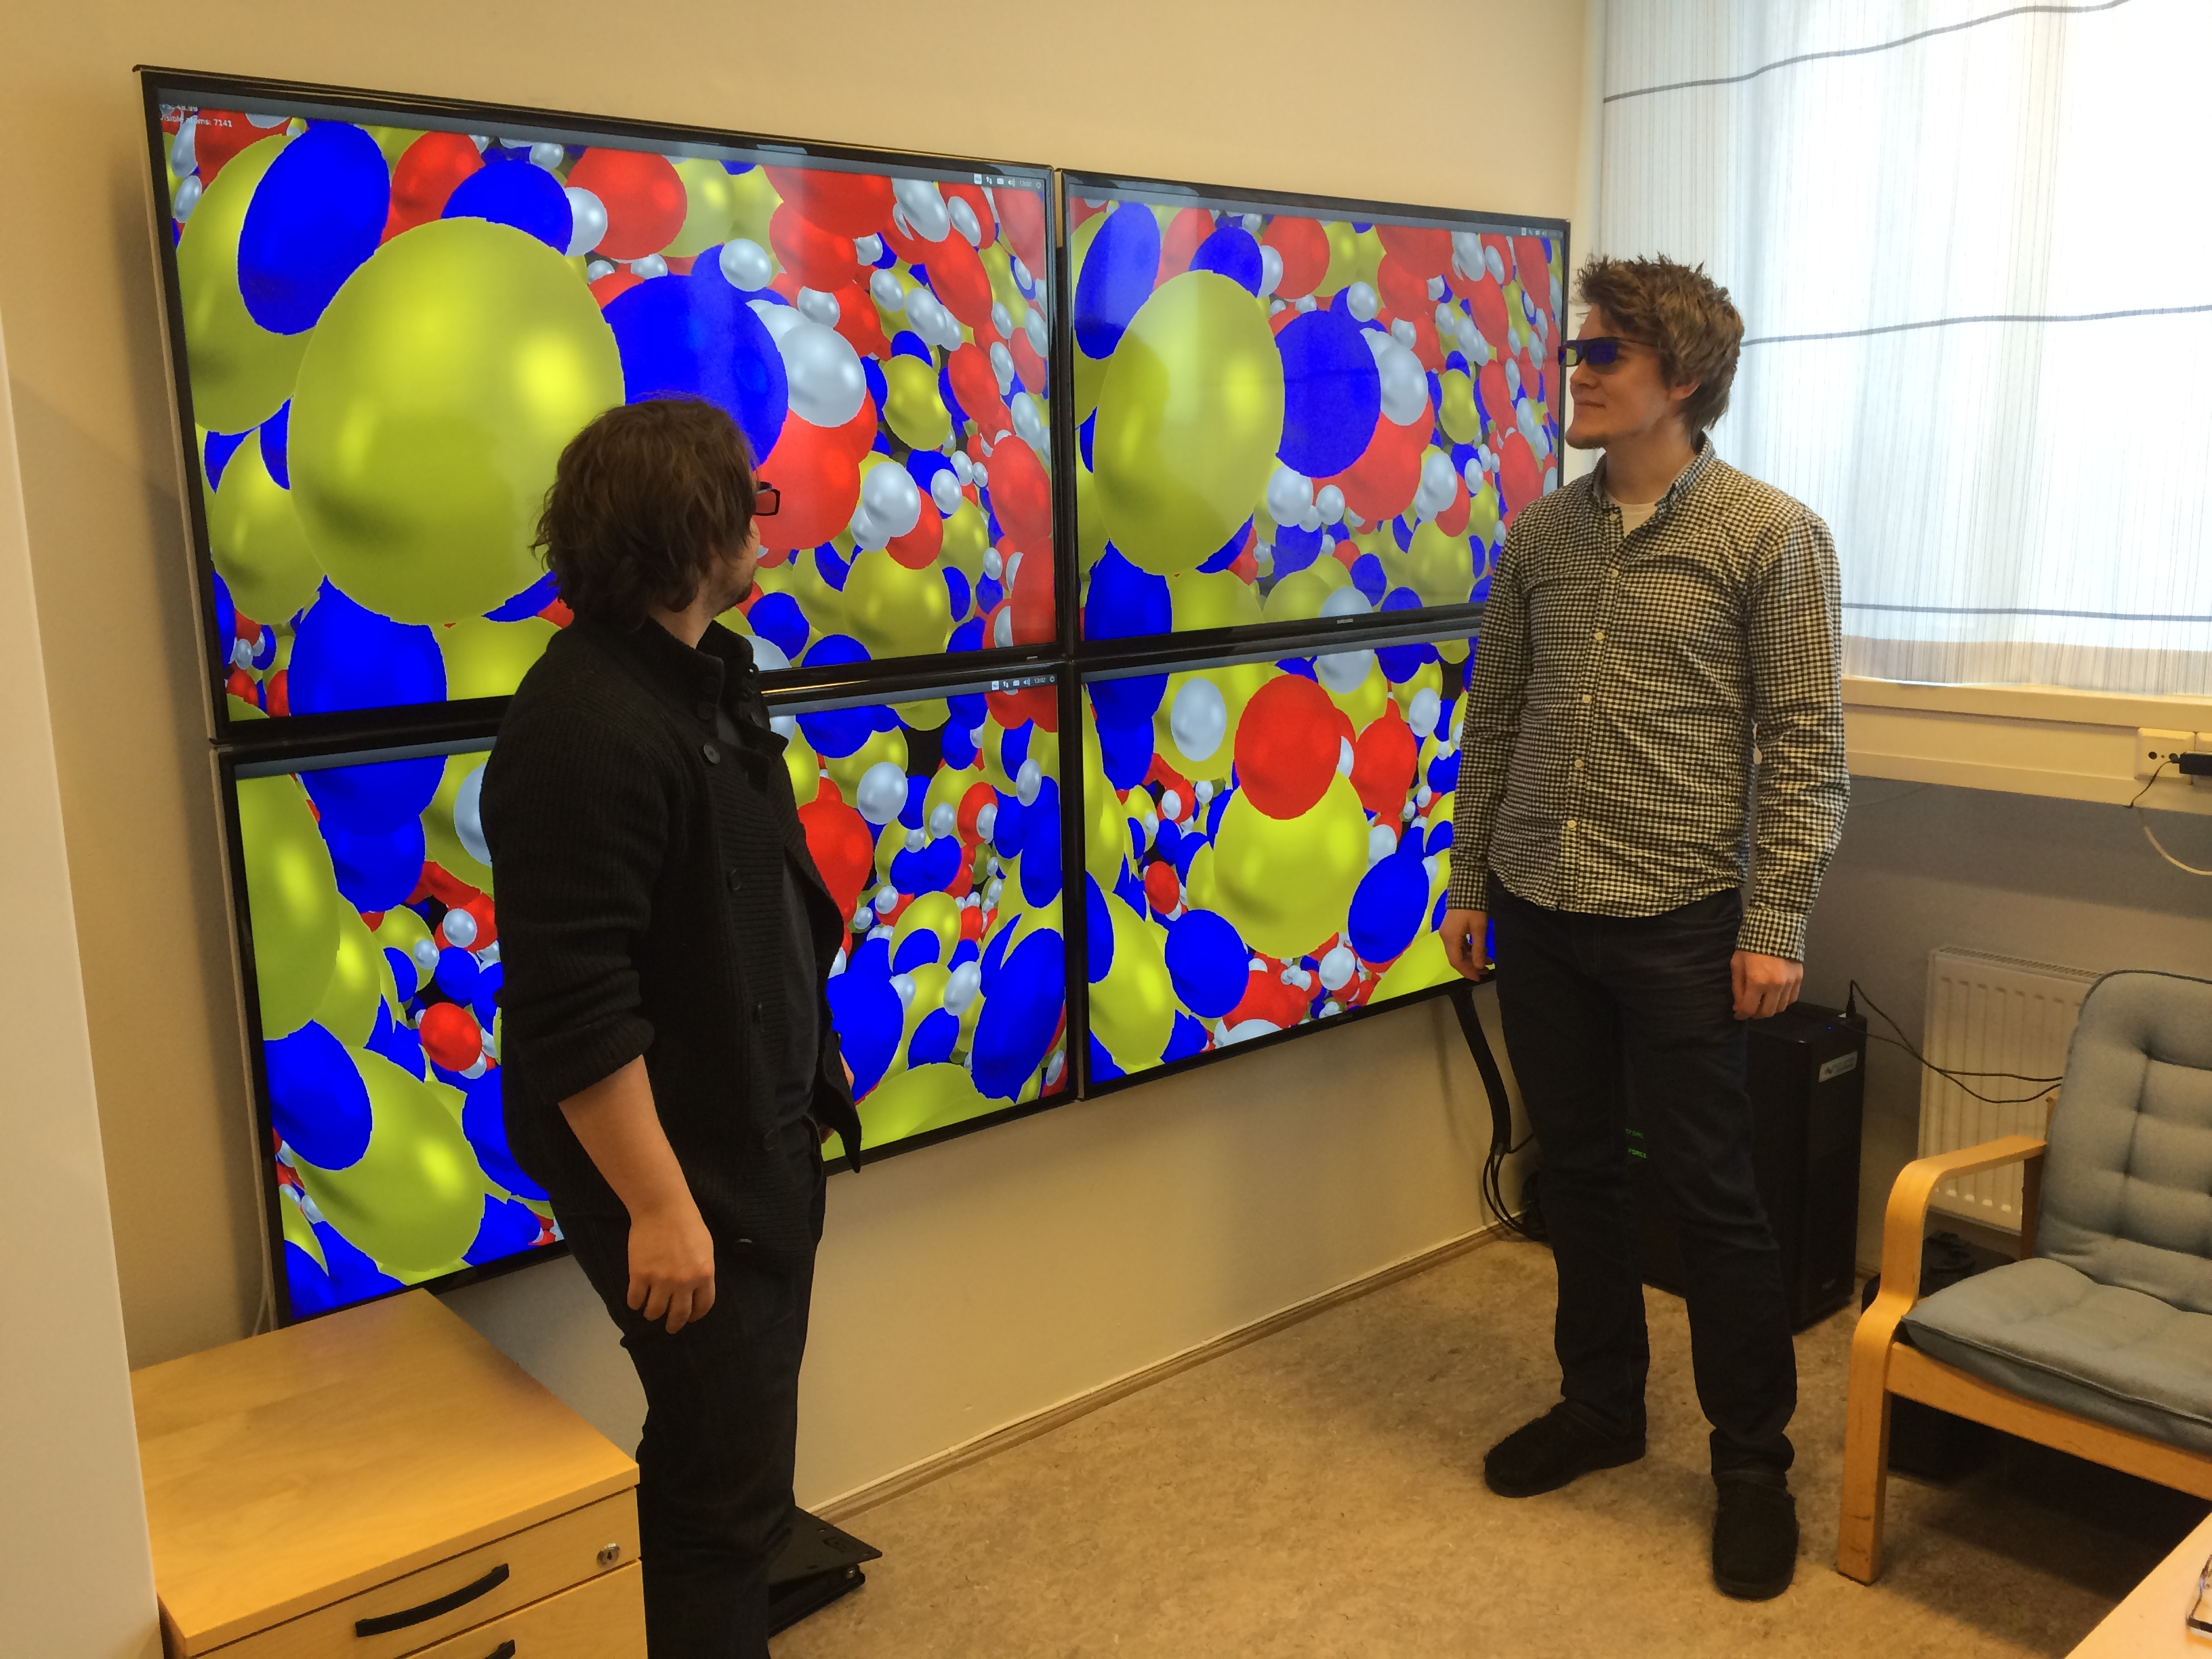
\includegraphics[width=1.0\linewidth]{fig-future/visualize.jpg}}


% !eslidecell




% !split
\subsection{Building a local supercomputing cluster from titan.uio.no}
% !bslidecell 00 0.2

% --- begin paragraph admon ---
\paragraph{Our supercomuting cluster.}
When UiO's previous supercomputing cluster (titan.uio.no) was replaced by \textbf{abel.uio.no}, we got 200 nodes for free from USIT and built our own supercomputer. The value in 2006 of all the equipment was close to eight MNOK.
\begin{itemize}
\item It helps students run and develop programs for large-scale problems locally

\item A successful program can then run on larger national and international supercomputers

\item Students run and maintain the local supercomputer

\item Used in regular courses as well
\end{itemize}

\noindent
% --- end paragraph admon ---


% !eslidecell

% !bslidecell 01 0.8


% inline figure
\centerline{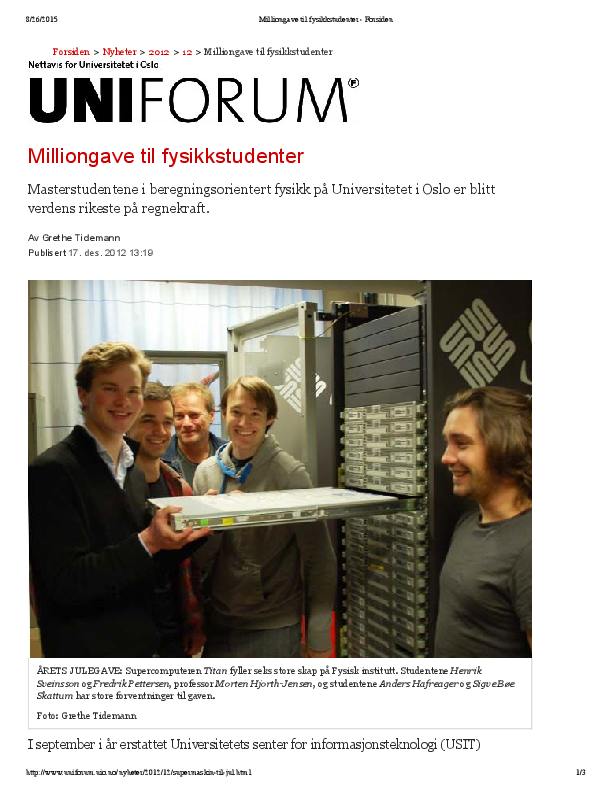
\includegraphics[width=1.0\linewidth]{fig-future/uniforum-0.png}}


% !eslidecell


% !split
\subsection{Undergraduate student publishes in PNAS}
% !bslidecell 00 0.1

% --- begin paragraph admon ---
\paragraph{Participating in research from day one!}
\begin{itemize}
\item Bachelor and master students publish in scientific journals 

\item Undergraduate students are exposed to research at early stages, often working with more advanced students

\item Students are exposed to all stages of the scientific process

\item Projects are tailored to the interests of the students

\item Focus on insights and sharing knowledge
\end{itemize}

\noindent
% --- end paragraph admon ---


% !eslidecell

% !bslidecell 01 0.9


% inline figure
\centerline{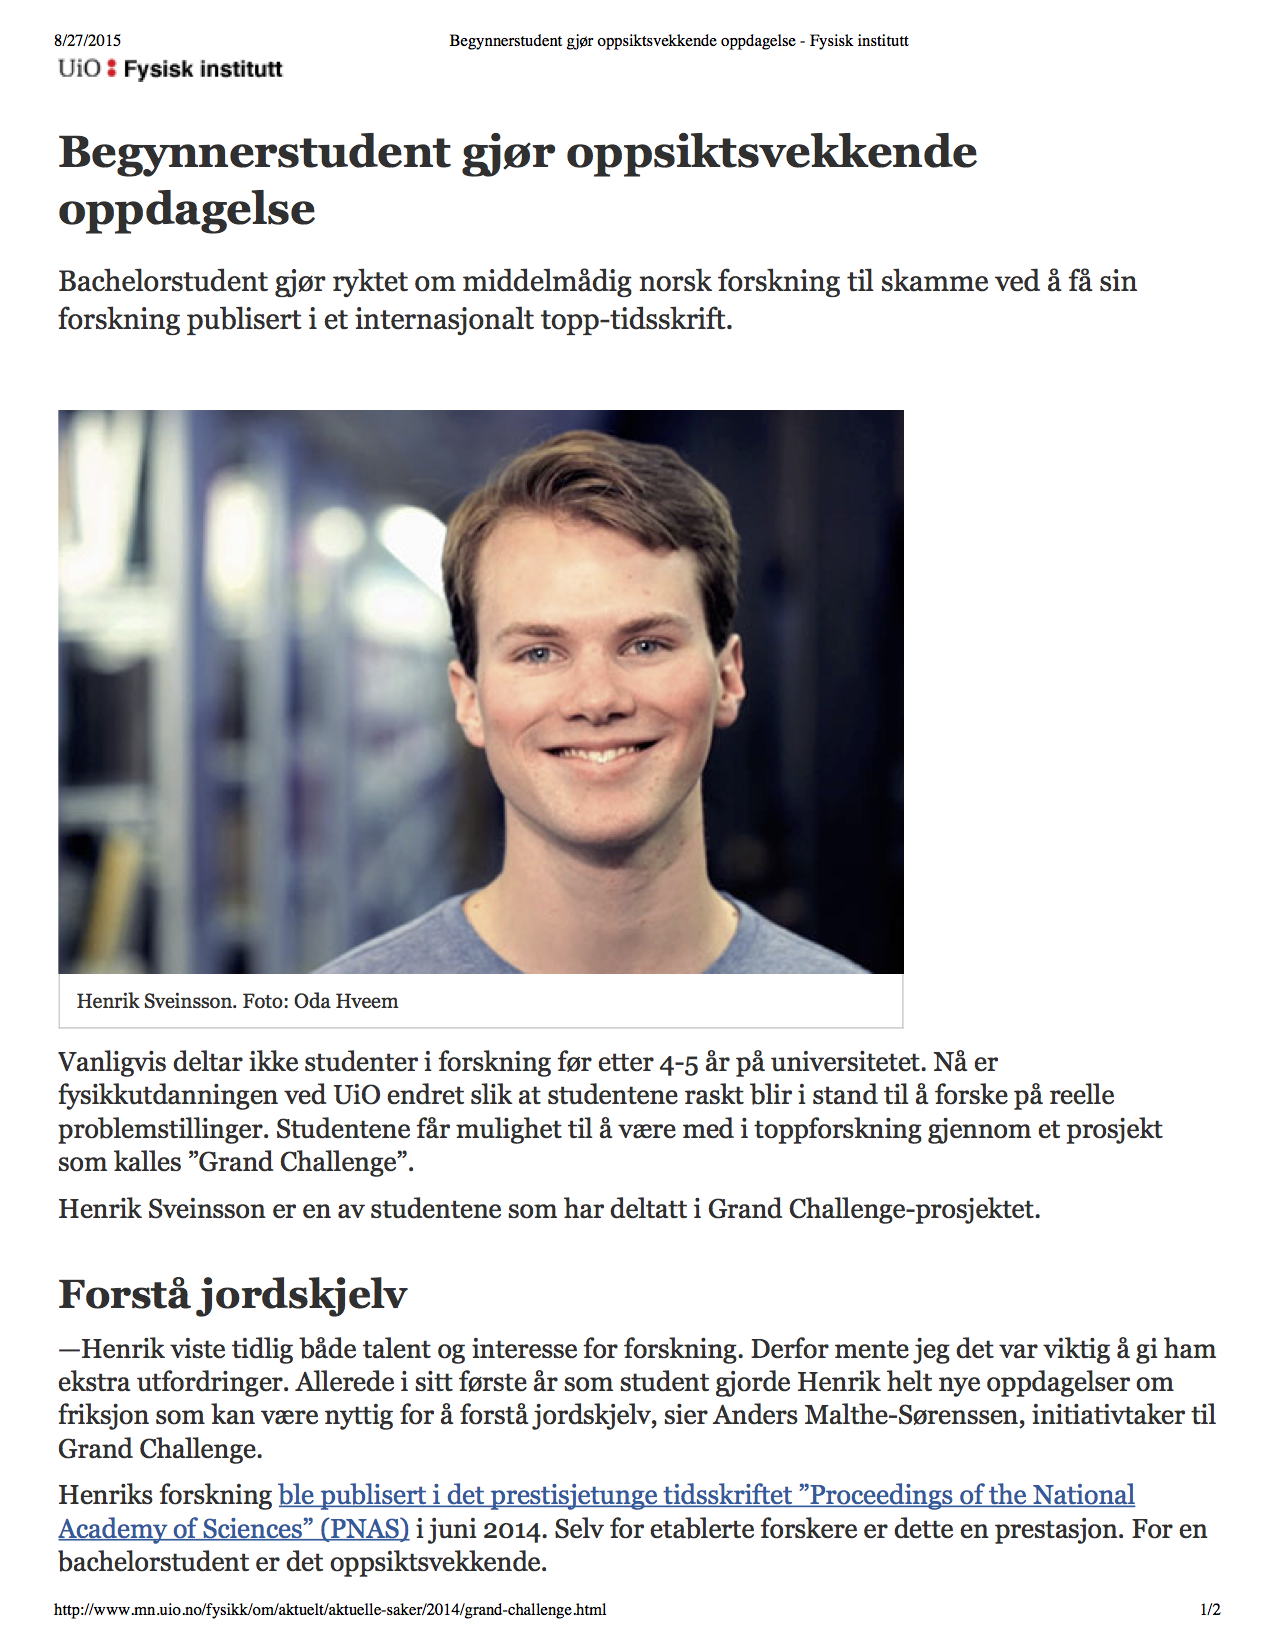
\includegraphics[width=1.0\linewidth]{fig-future/pnas.png}}


% !eslidecell






% !split
\subsection{Multiscale modeling is the big open research question in the 21st century}


% --- begin paragraph admon ---
\paragraph{}
\begin{itemize}
\item Present and future problems, unlike traditional
  science and engineering, involve complex systems with many distinct
  physical processes

\item The wide open research topic of this century, both in industry and at universities, is how to effectively couple processes across different length and energy scales

\item Progress will rely on a \emph{multi-disciplinary} approach
\end{itemize}

\noindent
% --- end paragraph admon ---




% --- begin paragraph admon ---
\paragraph{}
We need to foster candidates with the right
multi-disciplinary background and computational thinking!
% --- end paragraph admon ---




% !split
\subsection{The future: A new type of students}


% --- begin paragraph admon ---
\paragraph{}
\textbf{Computations will play a central role in almost all aspects of scientific investigations and technological innovation}
% --- end paragraph admon ---




% --- begin paragraph admon ---
\paragraph{}
\textbf{Candidates who are capable of modeling and understanding complicated systems, are in short supply in society}.
% --- end paragraph admon ---



% --- begin paragraph admon ---
\paragraph{}
We need students that
\begin{itemize}
\item can handle large and demanding multi-disciplinary  projects. This requires structured thinking and good analytical skills and a thorough understanding of the problems to be solved
\end{itemize}

\noindent
This knowledge makes the students unique on the labor market, a labor market which in the years to come will experience heavy automatization and massive loss of jobs.
% --- end paragraph admon ---



% --- begin paragraph admon ---
\paragraph{}
This will lay the foundation for cross-disciplinary
educational, research and innovation activities.
% It will contribute to building a common cross-disciplinary
% approach to key strategic initiatives, with important examples from fields like
% \emph{Energy research, Materials science and  Life Science}.
% --- end paragraph admon ---







% !split
\subsection{Create the Department for Computational Science!}


% --- begin paragraph admon ---
\paragraph{}
UiO's strength in computational science (education and research)
has the potential to make UiO a top European university
% --- end paragraph admon ---




% --- begin paragraph admon ---
\paragraph{How to achieve it.}
\begin{itemize}
\item Establish  a new center/department with focus on computational science and its applications to a wide range of fields (natural science, medicine, social sciences, humanities, applied research etc)

\item Hire ten young professors (age $< 40$) dedicated to innovative \emph{computational} research and education

\item Establish another ten professorships with  shared positions between the  new department and the discipline-specificdepartment (physics, chemistry, ...)
\end{itemize}

\noindent
% --- end paragraph admon ---



\textbf{The process must start now} in order not to lose momentum.



% !split
\subsection{Our takeaway messages}

% --- begin paragraph admon ---
\paragraph{}
\begin{itemize}
\item Computing plays and will play an even more important role in future scientific and technological advances

\item A successful research program cannot be disconnected from education and vice versa

\item An educational and research program which focuses on these issues needs to be established as soon as possible

\item Key goal: students must realize their own potentials and creative power
\end{itemize}

\noindent
% --- end paragraph admon ---




% !split
\subsection{Computational Physics and  the Computing in Science Education project (UiO educational prize in 2011)}


% --- begin paragraph admon ---
\paragraph{}
The results, insights, ideas and thoughts presented here, would have been impossible without the continuous interaction with colleagues in the \href{{http://www.mn.uio.no/english/about/collaboration/cse/}}{Computing in Science Education} project.
% --- end paragraph admon ---


% !bslidecell 00 0.4

% --- begin paragraph admon ---
\paragraph{}
\begin{itemize}
\item Hans Petter Langtangen

\item Knut Mørken

\item Arnt Inge Vistnes

\item Oyvind Ryan

\item Solveig Kristensen and Annik Myhre

\item Hanne Sølna

\item \textbf{And: all our fantastisc students who keep giving us new insights!}
\end{itemize}

\noindent
% --- end paragraph admon ---


% !eslidecell

% !bslidecell 01 0.6


% inline figure
\centerline{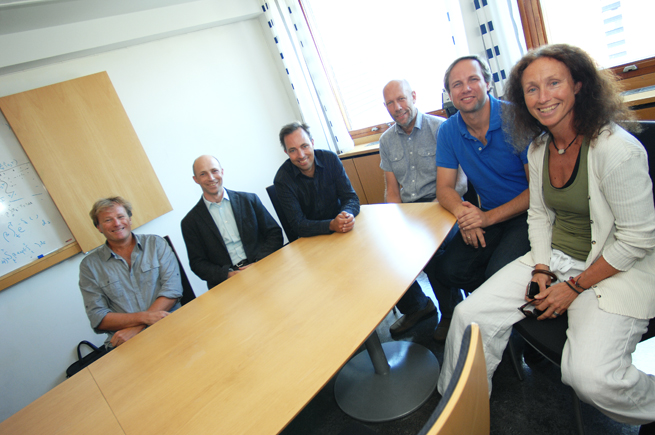
\includegraphics[width=1.0\linewidth]{fig-future/thegang.jpg}}


% !eslidecell







% ------------------- end of main content ---------------


% #ifdef PREAMBLE
\printindex

\end{document}
% #endif

